\section{Automatic $hp$-adaptivity}

The major difference between adaptivity in standard FEM and adaptivity
in $hp$-FEM is the large number of element refinement options in the
latter case. In standard $h$-adaptivity, elements can only be subdivided in space,
e.g., using the {\em red-green} refinement technique (see \cite{aksoylu} and the
references therein). In $hp$-adaptivity, one can either increase the polynomial
degree of elements without subdividing them in space or one can split elements
in space and distribute the polynomial degree on the subelements in multiple ways.

\subsection{Reference solution}

The presence of many $hp$-refinement options per element implies that
classical error estimates (in the form of one number per element)
do not provide enough information to guide $hp$-adaptivity. Instead,
one needs to use some information about the {\em shape} of
the error function $e_{h,p} = u - u_{h,p}$. In principle, this information
could be obtained by estimating higher derivatives, but such approach
is not very practical. Usually it is more convenient to use
a {\em reference solution}, i.e., an approximation $u_{ref}$ which is
at least one order more accurate than the coarse mesh solution $u_{h,p}$.
The $hp$-adaptivity is then guided by an a-posteriori error estimate
of the form
\be\label{errest}
e_{h,p} = u_{ref} - u_{h,p}
\ee

Such approach, as opposed to classical error estimates, is virtually
equation-independent. In this work we are constructing the enriched
finite element space by uniform subdivision of all mesh elements and 
by increasing all element polynomial degrees by one, i.e.
\bd
  u_{ref} = u_{h/2,p+1}
\ed

The reference solution $u_{ref}$ can be obtained efficiently by
utilizing information about lower frequencies from $u_{h,p}$
\cite{demk1,SoDe,solin1} if iterative solvers are used or by 
reconstructing the LU decomposition of the stiffness matrix
from the LU-decomposed coarse mesh stiffness matrix when using
direct sparse solvers, e.g. UMFPACK. However, we have not
attempted any such optimization in this work, even though we
admit that this issue must be addressed in order for the methods
to be usable in practice.


\subsection{Outline of the algorithm}

The outer loop of our adaptivity algorithm is formally similar
to the one of L.~Demkowicz et al. (see \cite{derade}), with minor
differences. The outline of the algorithm is as follows:
\begin{enumerate}
\item Assume an initial coarse mesh $\Tau_{h,p}$ consisting of piecewise-constant, linear or
      quadratic elements. User input includes
      \begin{enumerate}
			\item prescribed relative tolerance $TOL > 0$ for the
			      rate of energy norm of the approximate error function (\ref{errest}) and energy norm of the approximate solution 
			\item threshold ERRT specifying how many elements should be refined in each $hp$-adaptivity step
		\end{enumerate}
\item User input may also include
		\begin{enumerate}
			\item maximum increase of degrees of freedom $MAX\_STEP\_NDOF$ in each adaptivity step\\OR\\
			\item maximum number of degrees of freedom $MAX\_NDOF$
      \end{enumerate}

\item Create a fine mesh, $\Tau_{h/2,p+1}$

\item Compute fine mesh approximation $u_{h/2,p+1} \in V_{h/2,p+1}$ on $\Tau_{h/2,p+1}$.

\item Project the fine mesh approximation onto the coarse mesh $\Tau_{h,p}$. In this way, obtain a coarse mesh approximation.

\item Calculate the desired norm ($H^1$ norm, $H^1$ seminorm, $L^2$ norm, custom norm) of the fine mesh approximations $NORM_i$ on every element $K_i$ in the mesh, $i = 1, 2, \ldots, M$. Construct the approximate error function (\ref{errest}) as the difference between the fine and coarse mesh approximations, calculate its energy norm $ERR_i$ on every element $K_i$ in the mesh, $i = 1, 2, \ldots, M$. Calculate the global error estimate $$ERR = \lo\sum_{i=1}^M ERR_i\ro / \lo\sum_{i=1}^M NORM_i\ro.$$
      
\item If $ERR \le TOL$, stop computation and proceed to postprocessing.

\item Sort all elements into a list $L$ according to their value $ERR_i / NORM_i$
      in decreasing order.
      
\item Determine the maximum of element errors, $ERR_{max} = \max\{ERR_i / NORM_i\}$,
      by taking the first item of L.
      
\item Let {\it NDOF} be the current number of degrees of freedom of $\Tau_{h,p}$. Repeat the following cycle:
      \begin{enumerate}
			\item If $MAX\_STEP\_NDOF$ is set, and if the already added degrees of freedom in this $hp$-adaptivity step is greater than $MAX\_STEP\_NDOF$, break the cycle
      	\item Take the next element $K_i$ from the list $L$
      	\item If $ERR_i / NORM_i < ERRT \cdot ERR_{max}$, break the cycle
      	\item Perform $hp$-refinement of $K_i$ (to be described in more detail below).
      	\item If $MAX\_NDOF$ is set, and if the total number of degrees of freedom is now greater than $MAX\_NDOF$, break
      	the cycle
      \end{enumerate}
      
\item Continue with step C.\\
\end{enumerate}

The crucial issue in the outer loop is determining how many elements should be refined.
In \cite{derade} all elements whose error $ERR$ is greater than 70\% of the maximum
error $ERR_{max}$ are taken (ie. $ERRT = 0.7$). This is a relatively conservative
choice which leads to good convergence curves, but may result in too many steps
of the algorithm, which should be avoided as the evaluation of $u_{ref}$ is very
expensive. Our experience shows that setting $ERRT$ as low as 15\% results
in equally good convergence curves for most problems, but achieved in much fewer
steps and in turn in much shorter time. Occasionally, however, the low value of
$ERRT$ may cause too many elements to be refined and thus we introduced the 
limit $MAX\_STEP\_NDOF$ of the number of degrees of freedom added in each step. Typically,
one should not increase the number of degrees of freedom in each step by a large number.

\subsection{Selecting optimal $hp$-refinement}

The algorithm for determining optimal $hp$-refinements in \cite{derade} is 
quite complex. Built upon the projection-based interpolation theory,
it first finds optimal $hp$-refinement of mesh edges using a 1D
version of the $hp$-adaptive algorithm. The edge refinements then
determine $h$-refinement of elements. Finally, best polynomial
degrees for element interiors are selected. Each step of the algorithm
represents a considerable implementation burden.

We have implemented a much simpler scheme, which is local in the sense
that element refinements are selected without regard to the refinements
of neighboring elements. For all elements $K\in \Tau_{h,p}$ of polynomial
degree $p$ picked by the outer loop we consider the following 
$N = 83$ $hp$-refinement options:
\begin{enumerate}
\item Increase the polynomial degree of $K$ to $p+1$ without spatial subdivision.
\item Increase the polynomial degree of $K$ to $p+2$ without spatial subdivision.
\item Split $K$ into four similar triangles $K_1, K_2, K_3, K_4$.
      Define $p_0$ to be the integer part of $(p+1)/2$.
      For each $K_i$, $1 \le i \le 4$ consider polynomial
      degrees $p_0 \le p_i \le p_0 + 2$.
\end{enumerate}
For each of these $N$ options we perform a standard e.g. $L_2$-projection
of the reference solution $u_{ref}$ onto the corresponding polynomial
space. The candidate with smallest projection error is selected
for $hp$-refinement of the element $K$.

Each of the $N$ projection problems requires the solution of a small
system of linear algebraic equations with a symmetric positive-definite
matrix. The solution of these systems can be further optimized by exploiting
the incremental nature of the Cholesky decomposition algorithm 
and the fact that the spaces in item 3 above are partially embedded.
\paragraph{Example}
We again solve the model problem~\eqref{ade} with the same settings as in Paragraph~\ref{par:model_example}. This time, automatic hp-adaptivity will be used. Although the maximum value of the exact solution is $1.0$, due to the presence of undershoots and overshoots, the maximum values here are higher, as was seen already in section~\ref{sec:DG}. This can be avoided by using a suitable shock capturing method, as it is done in the last chapter with numerical examples for the Euler equations.
\begin{figure}[H]
\begin{center}
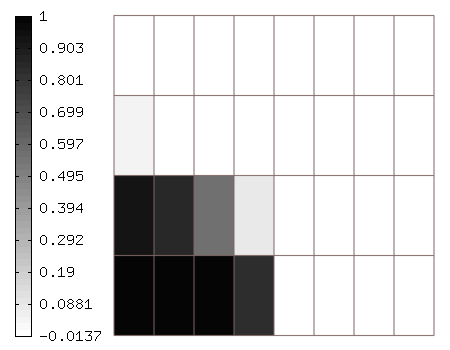
\includegraphics[width=0.48\textwidth]{minor_examples/Sln1.png}\ \ \ 
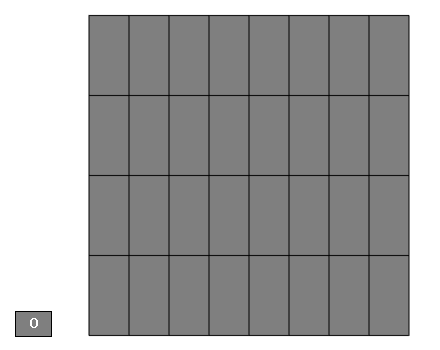
\includegraphics[width=0.48\textwidth]{minor_examples/Space1.png}
\end{center}
\vspace{-4mm}
\caption{Solution and a mesh, relative error between the fine mesh and the coarse mesh approximation: 25.7746\%.}
\end{figure}

\begin{figure}[H]
\begin{center}
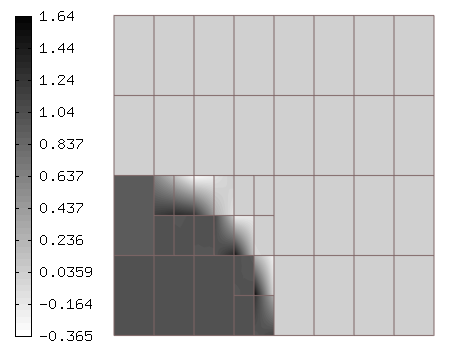
\includegraphics[width=0.48\textwidth]{minor_examples/Sln2.png}\ \ \ 
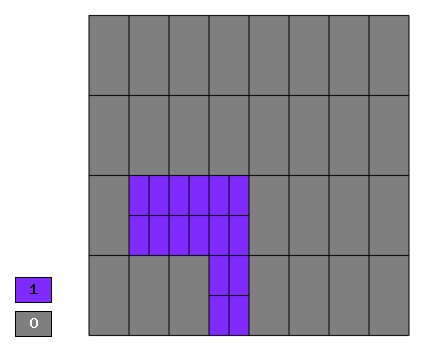
\includegraphics[width=0.48\textwidth]{minor_examples/Space2.png}
\end{center}
\vspace{-4mm}
\caption{Solution and a mesh, relative error between the fine mesh and the coarse mesh approximation: 10.3565\%.}
\end{figure}

\begin{figure}[H]
\begin{center}
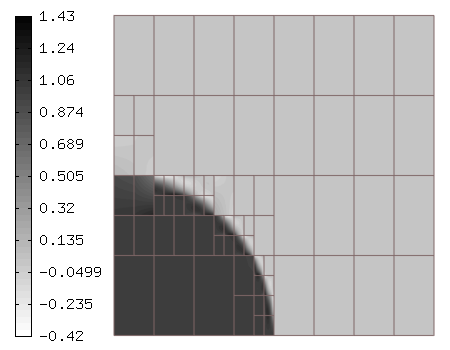
\includegraphics[width=0.48\textwidth]{minor_examples/Sln3.png}\ \ \ 
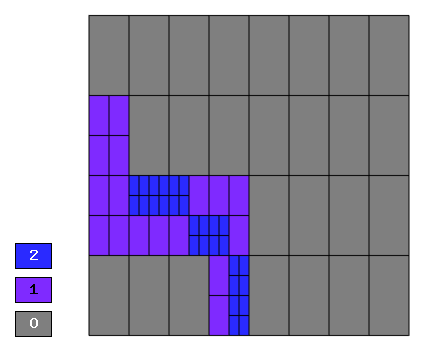
\includegraphics[width=0.48\textwidth]{minor_examples/Space3.png}
\end{center}
\vspace{-4mm}
\caption{Solution and a mesh, relative error between the fine mesh and the coarse mesh approximation: 5.58551\%.}
\end{figure}

\begin{figure}[H]
\begin{center}
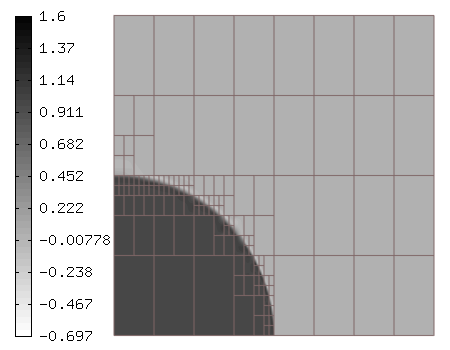
\includegraphics[width=0.48\textwidth]{minor_examples/Sln5.png}\ \ \ 
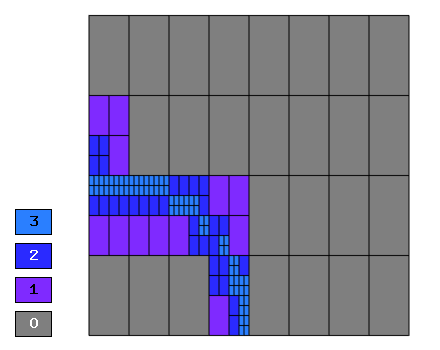
\includegraphics[width=0.48\textwidth]{minor_examples/Space5.png}
\end{center}
\vspace{-4mm}
\caption{Solution and a mesh, relative error between the fine mesh and the coarse mesh approximation: 2.43584\%.}
\end{figure}

\begin{figure}[H]
\begin{center}
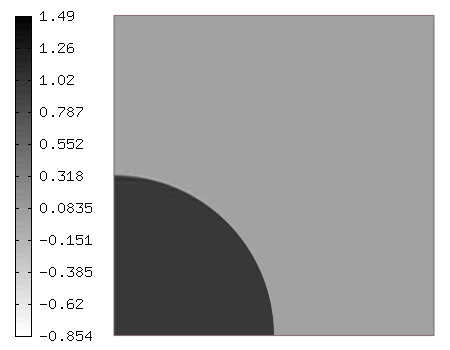
\includegraphics[width=0.48\textwidth]{minor_examples/Sln7.png}\ \ \ 
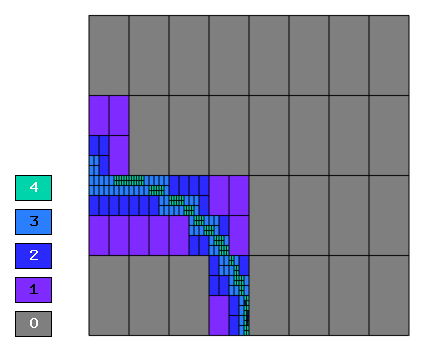
\includegraphics[width=0.48\textwidth]{minor_examples/Space7.png}
\end{center}
\vspace{-4mm}
\caption{Solution and a mesh, relative error between the fine mesh and the coarse mesh approximation: 1.27544\%.}
\end{figure}

\begin{figure}[H]
\begin{center}
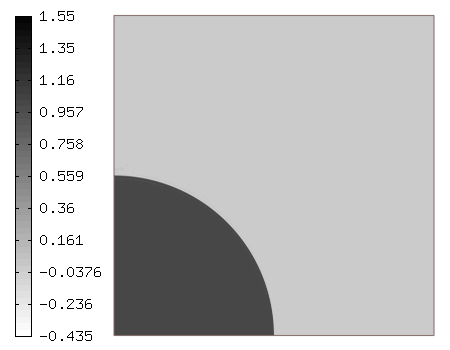
\includegraphics[width=0.48\textwidth]{minor_examples/Sln9.png}\ \ \ 
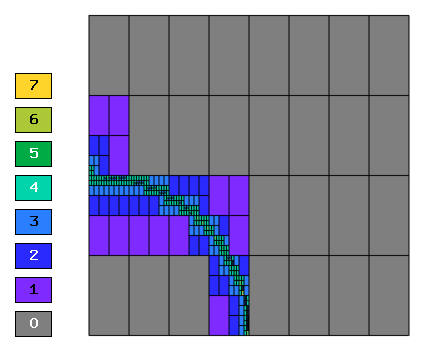
\includegraphics[width=0.48\textwidth]{minor_examples/Space9.png}
\end{center}
\vspace{-4mm}
\caption{Solution and a mesh, relative error between the fine mesh and the coarse mesh approximation: 0.919277\%.}
\end{figure}
